% Note that if you want something in single space you can
% go back and forth between single space and normal space
% by the use of \ssp and \nsp.  If you want doublespacing
% you can use \dsp.  \nsp is normally 1.5 spacing unless you
% use the doublespace option (or savepaper option)

\chapter{INTRODUCTION}
\label{c:intro}

This is the long example thesis produced by the  Department of
Mathematics and Statistics at San Diego State University
as a guide to using the \LaTeX\ template created by the Department.
It complies with the SDSU Thesis Manual produced in 2004
\cite{SDSUthesismanual}. 
The Department has created a \LaTeX\ class file that automatically
handles the formatting requirements of the SDSU Thesis Manual.  The
class file, the source file for this example thesis and for a shorter,
example thesis with more basic information, along with several other
materials are bundled together and available for distribution at
\cite{SDSUMath_thesis}. 

\section{Purpose}
\label{s:purpose}
This document  illustrates some of the more complex typesetting tasks
that are commonly encountered in a thesis containing mathematics.
The student should consult the  short example thesis
accompanying this distribution for information on more basic questions 
concerning the use of \LaTeX. All theses 
must follow the guidelines of the  SDSU Thesis Manual for formating. 
Most formating issues will be automatically handled by the \LaTeX\
class file included with the source file for this document, but there
may be some special circumstances that will require some tinkering
with spacing, pagebreaks, etc.

For a general reference it is recommended that the
student obtain the user's guide and reference manual of Leslie Lamport
\cite{LAM}. Another book that has been recommended is {\em Math into
  \LaTeX\ } \cite{Gra}. 
There are also numerous online resources:  For a general and polished
introduction see \cite{indian_tutorial}; For a focus on mathematics
see \cite{uiuc_tutorial}; For a focus on chemistry and biology see
\cite{microbio_resources}.
 The student should obtain copies of the files used to
generate this document and compare the ASCII source files with 
the \LaTeX\ output.

\section{The long example thesis}
\label{s:long}
The files for this long example
thesis are the following.
\begin{itemize}
\item {\tt sdsu-thesis.cls}: Defines the layout and formatting.
\item {\tt dchem.sty}: A package for doing chemistry.
\item {\tt thesis.tex}: 
\begin{enumerate}
\item  Contains information for the title page, and other
front-matter.
\item Contains a command to include the material from  the files 
{\tt abstract.tex},  {\tt body.tex}, and {\tt append.tex}.
\item Defines the bibliographical style (``plain'' in this example)
  and creates the bibliography using the file {\tt thbib.tex}. 
\end{enumerate}
\item {\tt abstract.tex}: Contains the abstract.
\item {\tt body.tex}: Contains all the text for chapters. 
\item {\tt append.tex}: Contains all the text for appendices.
\item {\tt thbib.bib}:  Contains a bibliographical database.
\item {\tt somb.eps}, {\tt cos.eps}, {\tt plot2.eps}, {\tt
  mol.cloud.ps}:  
Encapsulated postscript files 
that are included by {\tt body.tex}.
\item {\tt Makefile} This can be used on a unix/linux platform to
simplify the processing of \LaTeX/ files.
\end{itemize}

After processing these files the format of the thesis should comply
with the SDSU Thesis Manual.  The numbering of chapters, sections,
theorems, and bibliographical entries and any referencing to these
items should be correct.  Tables and figures are automatically placed
by \LaTeX, subject to certain constraints that you can provide.  
Occasionally, you may find  \LaTeX\ does not break a page or line  you
want it too, or you'd like to add vertical or horizontal space.
The command {\tt $\backslash$hspace\{1in\}} adds horizontal space and
{\tt $\backslash$vspace\{1in\}} adds vertical space.  You may also use
{\tt pt} (points) or {\tt cm} as 
measurements.  The  starred form {\tt $\backslash$hspace*\{12pt\}} of the command
is more persuasive than the unstarred form.  For breaking a line
{\tt $\backslash$newline} or {\tt $\backslash$linebreak} and for
breaking a page {\tt $\backslash$clearpage}, {\tt $\backslash$pagebreak}, {\tt
  $\backslash$newpage} are used, with subtle differences between these
commands (see a good reference). 


\chapter{THE EXCITING WORLD OF EQUATIONS,
THEOREMS, FIGURES AND TABLES}
\label{c:main}
In this chapter we see how equations, theorems,
figures and tables are created, enumerated and referenced.
Each of these items may be given a label
using {\tt $\backslash$label\{<labelname>\}}).
The item can then be referred to by {\tt
$\backslash$ref\{<labelname>\}}).
To see how any one of the examples is created, see the source file {\tt body.tex}.

We also play around with lengths of chapter and section headings.
For example, this chapter begins with a long chapter heading that must conform to the
thesis manual.  Later on there is a very long section heading.  These
examples show how the SDSU thesis class file automatically handles
formating.

We will occasionally refer to the {\it preamble} of the document.
This is set of  lines between the \LaTeX\
commands {\tt $\backslash$documentclass} and {\tt $\backslash$begin\{document\}}.
You may add or alter commands in the preamble to use supplementary
packages.  You can also use commands for a number of other things, as
we describe below.


\section{Equations}
\label{s:equations}
Within a line, mathematics is typeset using two dollar signs, \$, to
enclose the mathematical formula. For example $x_1^2 = x_{i_2}$.
Braces, \{ and \}, are used to help \LaTeX\ parse the input.
For displayed equations you may enclose the material with \verb+\[+
and \verb+\]+.
\[
I^e=\{f\in A\mid
\varphi(f)_i =0\ \forall i \mathrm{\ such\ that\ }
e_i\not=0\}.
\]
You may also use {\tt $\backslash$begin\{equation\}} and  {\tt
  $\backslash$end\{equation\}}. 
Here is a general differential equation,
\begin{equation}
\dot{x} = f(t,x),\qquad x(0)= x_0. \label{de1}
\end{equation}
To see that the numbering is going fine we insert a matrix system as
follows:
\begin{equation}
\dot{y} =
\begin{bmatrix}
a_1 & 0 & \cdots & 0 \\
0 & a_2 & \cdots & 0 \\
\vdots & \vdots & \ddots & \vdots \\
0 & 0 & \cdots & a_n
\end{bmatrix}
y.
\label{de2}
\end{equation}
The numbering is valuable when one wants to refer to the
Equations~(\ref{de1}) and~(\ref{de2}). You may also use abbreviations,
Eqn.~\eqref{de1} and~\eqref{de2}, but you should be consistent
about using one or the other.
Note that when referring to
Eqn.~(\ref{de1}) you must capitalize as we have
and it is best to type 
 a $\tilde{\phantom{x}}$ between the word Eqn., and the reference to avoid
inappropriate division of the label at the end of a line.

Notice that a displayed equation defined using  \verb+\[+ and
\verb+\]+, like the first equation above,  is not numbered. 
One may also  suppress numbering by using the starred form of the
{\tt equation} environment.
{\em e.g.}  {\tt $\backslash$begin\{equation*\}}.
\begin{equation*}
\dot{y} = g(y),
\end{equation*}

There are several other environments for displayed equations (each
having a starred form to suppress numbering). The {\tt align}
environment is useful for multiline equations or formulas.  It  requires an
ampersand in each line and uses it to align the formulas.
Here is the parameterization of the tangent surface to the twisted
cubic curve in 3-space.
\begin{align}
 k[x,y,z] &\longrightarrow k[t,u] \\
x & \longmapsto t + u \notag \\     %notice the placement of \notag
y & \longmapsto t^2 + 2tu \notag \\ %before the \\.
z & \longmapsto t^3 + 3t^2u \notag
\end{align}
Notice that all but the first line have a {\tt $\backslash$notag}
command to suppress numbering. 

There is also an {\tt alignat} environment that allows you to align
more than one equation in a row and add extra space between the equations.
\begin{alignat}{2}
\label{e:rho lam}
\rho(e_i) &= \rho(f_i) & \qquad \lambda(e_i) &= \lambda(f_{i-1}) 
\intertext{I can even add some text between the two rows.}
\rho(e'_i) &= \rho(f'_i) & \qquad \lambda(e'_i) &= \lambda(f'_{i-1}) 
\end{alignat}

Here are a couple of other useful examples
\[
\delta_{ij} = \begin{cases}
1 & \text{if $i=j$} \\
0 & \text{else}
\end{cases}
\]
For $f(x)= \prod_{i=1}^n (x-\alpha_i)$ we have
\[ 
f'(x) = 
\sum_{i=1}^n \prod_{\substack{j=1 \\j \not= i}} ^n (x-\alpha_j)
\]
You might want to label arrows
\[
X \stackrel{f}{\longleftarrow} Y
\]

\section{Theorems, etc.}
\label{s:theorems}
Modern mathematics texts are quite formal about enumerating theorems,
lemmas, definitions etc.  In this 
section we show how to do this with  \LaTeX.

\begin{definition}   
\label{d:stable}
A linear differential equation is asymptotically stable if and only if
all eigenvalues, $\lambda$, of the operator matrix have negative real
part.
\end{definition}
We follow this with a couple of theorems and a corollary.
\begin{theorem}
\label{t:lde}
If the matrix $A$ in the linear differential equation,
\begin{equation}
\dot{y} = Ay, \qquad y(0) = y_0, \label{lde}
\end{equation}
is symmetric, then the solution of {\rm (\ref{lde})} is non-oscillatory.
\end{theorem}
\begin{corollary}
\label{c:symmetric}
If the matrix $A$ in {\rm (\ref{lde})} is symmetric and has negative
eigenvalues, then the solution is non-oscillatory and asymptotically
stable.
\end{corollary}

In order to check how the numbering proceeds we insert here another
theorem.  Notice that Theorem~\ref{t:lde} is the first theorem.
\begin{theorem}
\label{t:antisymmetric}
If the matrix $H$ in the linear differential equation,
\begin{equation}
\dot{y} = Hy, \qquad y(0) = y_0, \label{ldeh}
\end{equation}
is antisymmetric, then the solution of {\rm (\ref{ldeh})} is oscillatory.
\end{theorem}

\begin{proof}
The proof is clear.
\end{proof}

You may choose alternate methods to enumerate theorem-like
environments.  For example, another method would be to use one counter
for all environments.  
In  the preamble at the  beginning of  {\tt thesis.tex} 
you will find the \LaTeX\ code to accomplish this.
You can choose a different method by altering the \LaTeX\ code.
You might also want to add other environments, such as an 
{\em example} environment or an {\em algorithm} environment.
Notice also the {\em proof} environment that nicely places the box at
the end of the proof and introduces the proof with Proof in italic.

\section{Figures or How to Get into Real Trouble if You Take Advantage
of What \LaTeX\ Can Do}
\label{s:figures}

This section shows how to display figures and refer to them in the text.
We will focus here on using \LaTeX\ to insert postscript files using the
{\tt epsfig} package.  Make sure to include
{\tt $\backslash$usepackage\{epsfig\} } in your preamble.

Suppose that we have a postscript file of the  graph of the curve
\begin{equation}
y=\sin(\omega t), \label{gr1}
\end{equation}
where $\omega$ is the circular frequency.
Figure~\ref{fig1} is a graph of Equation~(\ref{gr1}). The interval
of time viewed is $t \in [-5,5]$. The figure reference should be denoted
by either Fig.~\ref{fig1} or by Figure~\ref{fig1}.
\begin{figure}[htb]
\centering
\begin{minipage}{4.5in}
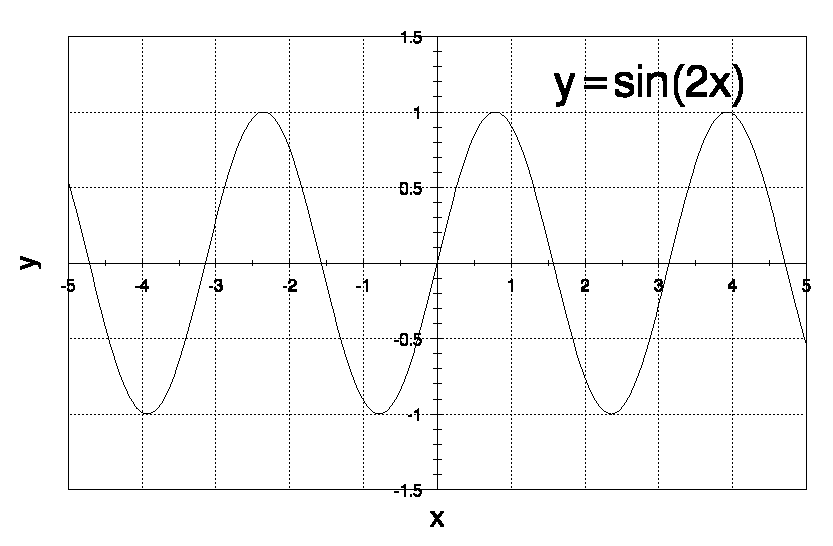
\epsfig{file=plot2.eps,width=4.5in}
\caption{This is a graph of the above equation, where the
circular frequency is taken as $\omega = 2$.\label{fig1}}
\end{minipage}
\end{figure}

This figure was created with a mathematics software package which
produced an encapsulated postscript file.  
In general, to insert  a file named {\tt fname.ps} you
do the following to include it in your thesis:
\\
{ \tt
\hspace*{0.5in} $\backslash$begin\{figure\}[htb]
\\
\hspace*{0.5in} $\backslash$epsfig\{file=fname.ps,height=$x$in\}
\\
\hspace*{0.5in} $\backslash$caption\{Insert a caption here. $\backslash$label\{figlabel\} \}
\\ 
\hspace*{0.5in} $\backslash$end\{figure\}
}
\\
The $x$ above is some number of inches.
This will left justify the figure.  Centering is
a little more complicated and you have to know the width of the figure.
So instead of specifying {\tt height} for the figure we specify
{\tt width}, place everything in a {\tt minipage} environment of that width
and center that.  For example (where $x$ would be some number again):
\\
{ \tt
\hspace*{0.5in} $\backslash$begin\{figure\}[htb]
\\
\hspace*{0.5in} $\backslash$centering
\\
\hspace*{0.5in} $\backslash$begin\{minipage\}\{$x$in\}
\\
\hspace*{0.5in} $\backslash$epsfig\{file=fname.ps,width=$x$in\}
\\
\hspace*{0.5in} $\backslash$caption\{Insert a caption here. $\backslash$label\{figlabel\} \}
\\
\hspace*{0.5in} $\backslash$end\{minipage\}
\\
\hspace*{0.5in} $\backslash$end\{figure\}
}

Fig.~\ref{fullfig} contains two different graphs included in one figure.

Note that if you cannot obtain
postscript figures or are having too much trouble using the technique
described above, then you can use the {\tt $\backslash$vspace}
command to provide an
empty space in the manuscript, then use the old-fashioned technique of
taping in your figure and photocopying it.



%
% If you have oversize full page figures, the following
% might come in handy
%
%\figurecoversheet{\label{figure:oversize} Caption goes here}


%%%%%%%%%%%%%%%%%%%%%%%%%%%%%%%%%%%%%%%%%%%%%%
%%%     The \hspace*{-0.5} moves the figure to the left a bit so that
%%%     it lines up with the caption.
%%%     The \newline seems to be necessary so that the second figure
%%%     lies below the first.
%%%%%%%%%%%%%%%%%%%%%%%%%%%%%%%%%%%%%%%%%%%%%%

\begin{figure}[htb]
\centering
\begin{minipage}{3.5in}
\hspace*{-0.5in}
\epsfig{file=somb.eps,width=3.5in}\newline
\hspace*{-0.5in}
\epsfig{file=cos.eps,width=3.5in}
\caption{The top graph is the function $z = \sin(r)/r$, while
the bottom surface is the function $z = \cos(r)$. \label{fullfig}}
\end{minipage}
\end{figure}

\section{Tables}
\label{s:tables}

The Department of Mathematical Sciences does not have specific
requirements on the exact layout of a table. However, the tables should
be easily readable and properly labeled according to the regulations in
the SDSU Thesis Manual. In this section we want to demonstrate how
\LaTeX\ handles tables. More complicated examples can be found in
Lamport's book \cite{LAM}. We begin with a small table, given by
Table \ref{tab1} which inserts nicely into the text.  Note that the same
centering trick as was employed for figures is done here and we set the
width of the {\tt minipage} environment to 1.9 inches.
%

\begin{table}[hbt]
\centering
\begin{minipage}{1.9in}
 \caption{A Small Table for Listing Some Parameters Used in Some
          Numerical Procedure\label{tab1}}
 \begin{tabular}{|c||c|c|c|c||}    \hline
  Trial &	a  &  b & c & $\omega$ \\ \hline \hline
  1 & 5 & 10  & 15 & $\pi$ \\ \hline
  2 & 10 & 20  & 15 & $2\pi$ \\ \hline
 \end{tabular}
\end{minipage}
\end{table}
%

The manual however allows for the caption to be a little wider if the table
is really small and so we can use a wider {\tt minipage} and then center
the table inside there.  See for example Table \ref{wtab} where we used
width of 3.5 inches.
%
\begin{table}[hbt]
\centering
\begin{minipage}{3.5in}
  \centering
  \caption{Another Small Table for Listing Some Parameters Used in a
           Numerical Procedure\label{wtab}}
   \begin{tabular}{|c||c|c|c|c||}    \hline
    Trial &	a  &  b & c & $\omega$ \\ \hline \hline
    1 & 5 & 10  & 15 & $\pi$ \\ \hline
    2 & 10 & 20  & 15 & $2\pi$ \\ \hline
   \end{tabular}
\end{minipage}
\end{table}

Note that you can use the {\tt center} environment instead of {\tt
$\backslash$centering} but that might add a little bit of unwanted
whitespace.  With {\tt $\backslash$centering} on the other hand, you
might have to put braces around the text you wish to center and
sometimes need to add a {\tt $\backslash$par}.  If you use it inside
a {\tt minipage}, {\tt table} or {\tt figure} environment, you don't have
to really worry about that.  Note however that without the use of
{\tt minipage} you cannot center the caption as it automatically left aligns
itself to conform with the thesis manual.

Tables can also be left aligned see for example Table \ref{ltab}.  Here we
don't use the {\tt minipage} environment, but we must then add linebreaks
so that the table caption does not go wider then the table itself.  We need
to add then two titles, one for the list of tables and one for the caption
here.  The former will not have line breaks and the latter will.
% The first caption (in brackets[]) is used for the list of tables.

\begin{table}[hbt]
 \caption[
   Another such table but left aligned.]{
   Another Such\\Table but Left Aligned\label{ltab}}
 \begin{tabular}{|c||c|c|c|c||}    \hline
  Trial &	a  &  b & c & $\omega$ \\ \hline \hline
  1 & 5 & 10  & 15 & $\pi$ \\ \hline
  2 & 10 & 20  & 15 & $2\pi$ \\ \hline
 \end{tabular}
\end{table}


You might also want to use an entire page for a long table,
This is done by typing the command $\backslash$begin\{table\}[p]. 

Here is an example, included in the minipage environment, to show how 
footnotes\footnote{We also need to see how a regular footnote
appears in the text, so one was inserted here. Multiple lines are easily
handled by \LaTeX.}
can be added to a table.
\begin{table}[bh]
\centering
\begin{minipage}{3.7in}
\caption{Computations for Products of the {\em rrn} Genes at Different
Growth Rates\label{tab2}}
\begin{tabular}{|c||c|c|c|c|c||}	 \hline
 $\tau$(min)  &  100  &	60 & 40 & 30 & 24 \\ \hline \hline
 $C$ period & 67 & 50  & 45 & 43 & 42 \\ \hline
 $D$ period & 30 & 27  & 25 & 24 & 23 \\ \hline
 $V_0$ & 0.437 & 0.577 & 0.815 & 1.15 & 1.63 \\ \hline
 $\bar c$\footnote{$\times 1000\ {\rm ribosomes}/\mu{\rm m}^3$.}
 & 11.1 & 16.8 & 22.1 & 28.1 & 31.4 \\ \hline
$\bar c_{85}$\footnote{$\times 1000\ {\rm ribosomes}/\mu{\rm m}^3$,
representing the average concentration of the product of the {\em rrn} gene
located at $85'$.} & 1.73 & 2.68 & 3.65 & 4.81 & 5.57 \\ \hline
$\bar c_{57}$\footnote{$\times 1000\ {\rm ribosomes}/\mu{\rm m}^3$,
representing the average concentration of the product of the {\em rrn} gene
located at $57'$.} & 1.36 & 1.98 & 2.43 & 2.87 & 2.96 \\ \hline
$\bar c_{85}({\scriptstyle\times 100})/\bar c$\footnote{Percentage of
$\bar c$ produced by the {\em rrn} gene located at $85'$.} & 15.6 & 15.9 &
16.5 & 17.1 & 17.7 \\ \hline
$\bar c_{57}({\scriptstyle\times 100})/\bar c$\footnote{Percentage of
$\bar c$ produced by the {\em rrn} gene located at $57'$.} & 12.3 & 11.8 &
11.0 & 10.2 & 9.44 \\ \hline
$\bar c_{85}/\bar c_{57}$ & 1.27 & 1.35 & 1.50 & 1.68 & 1.88 \\ \hline
 $r$\footnote{Initiations/min/gene.} & 3.75 & 10.27
  & 22.56 & 38.42 & 56.98 \\ \hline
$c_{max}$\footnote{$\times 1000\ {\rm ribosomes}/\mu{\rm m}^3$, representing
the maximum concentration during the cell cycle.} & 11.28 & 17.04
  & 22.33 & 28.36 & 31.77 \\ \hline
$c_{max}/c_{min}$\footnote{Ratio of maximum to minimum concentration
 during the cell cycle.} & 1.041 & 1.036 & 1.027 & 1.024 & 1.026 \\ \hline
\end{tabular}
\end{minipage}
\end{table}

%\clearpage
Sometimes a table might not fit onto a single page, in this case you
must not use the {\tt table} environment, but instead the {\tt longtable}
environment.  Do note that {\tt longtable} automatically centers so you need
not worry about that.  See Table \ref{totallyrandom} for some absolutely
random numbers.  To use the {\tt longtable} environment you must include the
{\tt longtable} package in your preamble.

\begin{longtable}{|l|l|l|}
% You may need to modify the \LTcapwidth if the title wraps too early, or
% if it makes your table too large
%\LTcapwidth=6in
\caption{A Table of Some Totally Random Numbers} \label{totallyrandom} \\

% Here are our column headings
\hline
\multicolumn{1}{|l|}{\textbf{First}} &
\multicolumn{1}{l|}{\textbf{Second}} &
\multicolumn{1}{l|}{\textbf{Third}} \\
\hline \hline
\endfirsthead

% Here is the caption on other pages
\caption*{\tablename\ \thetable{} (continued)} \\
\hline \multicolumn{1}{|l|}{\textbf{First}} &
\multicolumn{1}{l|}{\textbf{Second}} &
\multicolumn{1}{l|}{\textbf{Third}} \\ \hline \hline
\endhead

\multicolumn{3}{r}{\textbf{(table continues)}}
\endfoot

\hline
\endlastfoot

$16883.20050 \times 64.19591$ & $23174^{2905}$ & $(5112,5468,27117)$ \\ \hline
$7216.3398 \times 12239.16770$ & $19961^{9127}$ & $(16136,21997,26051)$ \\ \hline
$15977.29588 \times 5732.19698$ & $14995^{26728}$ & $(28634,14278,17183)$ \\ \hline
$24699.2338 \times 8803.18474$ & $19221^{28853}$ & $(18539,6044,19259)$ \\ \hline
$21444.11156 \times 24727.15793$ & $18372^{28126}$ & $(28032,2375,15319)$ \\ \hline
$4391.18511 \times 4548.30442$ & $1720^{1369}$ & $(3406,21419,16364)$ \\ \hline
$30135.17285 \times 30643.14550$ & $9216^{213}$ & $(23353,27690,19435)$ \\ \hline
$19438.13461 \times 25479.5929$ & $2137^{3868}$ & $(30657,17930,22240)$ \\ \hline
$26015.13194 \times 24615.8566$ & $17585^{10358}$ & $(13114,15259,12079)$ \\ \hline
$14483.18666 \times 730.30848$ & $16033^{18015}$ & $(28723,30583,27231)$ \\ \hline
$28936.21168 \times 22153.15603$ & $7838^{2847}$ & $(8315,13767,4984)$ \\ \hline$12183.11656 \times 22915.1655$ & $4903^{3341}$ & $(26271,13469,20927)$ \\ \hline
$3861.26584 \times 3418.15940$ & $8299^{22084}$ & $(16670,6379,5349)$ \\ \hline
$1917.2334 \times 3164.29148$ & $31271^{24332}$ & $(18534,14106,32170)$ \\ \hline
$21381.22421 \times 13170.26365$ & $1836^{24826}$ & $(16512,3492,29730)$ \\ \hline
$19854.29763 \times 10431.8013$ & $856^{4247}$ & $(11431,16797,12547)$ \\ \hline$748.699 \times 18926.6097$ & $2617^{21261}$ & $(9262,31765,19764)$ \\ \hline
$826.17531 \times 1102.229$ & $6144^{23524}$ & $(13399,32510,25360)$ \\ \hline
$5457.16254 \times 28852.2419$ & $3340^{25847}$ & $(12851,11353,26704)$ \\ \hline
$17098.22785 \times 10733.29645$ & $23533^{11432}$ & $(15804,29630,14049)$ \\ \hline
$4297.6124 \times 13047.24061$ & $6951^{30578}$ & $(25163,7180,3955)$ \\ \hline
$15919.20579 \times 3697.8512$ & $26036^{19951}$ & $(4596,28456,23292)$ \\ \hline
$30444.8539 \times 1877.24380$ & $25637^{24662}$ & $(2345,22515,15427)$ \\ \hline
$13777.5551 \times 12290.27827$ & $9848^{18414}$ & $(8106,1141,25365)$ \\ \hline$5916.26304 \times 32545.9871$ & $9456^{20356}$ & $(13568,17968,13625)$ \\ \hline
$752.22564 \times 9313.24044$ & $20240^{17852}$ & $(25921,11852,10721)$ \\ \hline
$17816.14197 \times 468.475$ & $27975^{6019}$ & $(12765,23034,15867)$ \\ \hline
$31180.31140 \times 17008.23777$ & $4288^{10545}$ & $(23555,14160,20001)$ \\ \hline
$11143.27728 \times 5201.24768$ & $28480^{27765}$ & $(1313,19756,15238)$ \\ \hline
$19165.12910 \times 27090.29887$ & $30726^{8520}$ & $(30355,31201,3727)$ \\ \hline
$3607.11199 \times 26761.19474$ & $9611^{25133}$ & $(3715,620,29421)$ \\ \hline
$14260.24175 \times 10813.1493$ & $2551^{5774}$ & $(6694,27319,1486)$ \\ \hline
$1691.28633 \times 21243.16929$ & $15030^{1385}$ & $(11252,12149,32111)$ \\ \hline
$19772.9737 \times 30544.23499$ & $13344^{8975}$ & $(17492,50,18586)$ \\ \hline
$9857.3765 \times 19207.6510$ & $18025^{10614}$ & $(17324,19518,13165)$

\end{longtable}


\chapter{CREATING A BIBLIOGRAPHY USING {\sc Bib}{\TeX} }
\label{c:biblio}
There are two ways to create a bibliography.  In the short example
thesis you enter the bibliographic items as they are supposed to
appear.  In this example thesis we show how to use {\sc Bib}\TeX.
With {\sc Bib}\TeX\ you create a separate file, {\tt thbib.bib} in our
example, containing data about each bibliographical item.
Here is an example,
\begin{verbatim}
@article{ART,
  author="Abraham, T.",
  title="Mathematical study of $\gamma$-rings in a {H}ilbert space",
  journal="J. Math. Anal. Appl.",
  volume="19",
  pages="125-128",
  year="1984"
}
\end{verbatim}
Here {\tt @article} describes the type of entry and {\tt ART} is the
tag that you use to cite the entry.
Running {\sc Bib}\TeX creates a file containing your bibliography in
\LaTeX\ format, {\tt thesis.bbl} in this example.  
You don't have to worry about alphabetizing,
enumerating, or  formatting. {\sc Bib}\TeX\ does all of that
automatically.  Furthermore, {\sc Bib}\TeX\ only includes items that
you have referenced in the thesis, so your database can include
extraneous entries.  {\sc Bib}\TeX\ also allows you to choose the 
bibliographical style  with one command, for example
{\tt \verb+\bibliographystyle{plain}+}, so it is easy to change from
one style to another.

MathSciNet has a nice feature that frees you from actually entering
the data. 
If you do a search for the item on MathSciNet, you will see a button
that says ``select alternative format.''  Choose {\sc Bib}\TeX\ and
you will get the bibliographical data.
There is also a clipboard on the  search page on which you can
store  data for several items.  Click ``Add citation to
clipboard'', below each item that you want.
You can see the items you've selected by clicking  on the link "View
clipboard" at the top left of  the page.
Select ``Bibtex'' as format, hit the ``Text'' button and you have the
data.  You will probably want to change the tags to something easy for
you to remember.

In the bibliographic database we have included  references for journal articles
\cite{ART}, books and booklets \cite{AM,BKL}, chapters or articles in
books, collections, and proceedings \cite{INB,INC,INP}. 
Other sources may be proceedings \cite{PRO},
technical reports \cite{TEC}, theses \cite{MTH}, or unpublished material
\cite{UNP}.  A number of online references are also given
\cite{uiuc_tutorial,indian_tutorial}.
This should provide a fairly comprehensive list for any
material that the student may encounter.  For additional assistance, see
the graduate adviser in your area of concentration.  

When you want to include a reference to a particular page, theorem
chapter or whatever, you can use an optional argument to the cite
command.  For example, \cite[Thm.~1.1]{AM}


\chapter{CHEMISTRY}
\label{c:chem}

For chemistry theses with many mathematical formulas, the 
{\tt   amsmath} package is  recommended. Simply use the line
{\tt $\backslash$usepackage\{amsmath\}} in the preamble.

To obtain the {\sc Bib}\TeX\ style file for formatting references in ACS style,
install the  following package.
\begin{description}
\item \verb+http://www.ctan.org/tex-archive/macros/latex/contrib/achemso+
\end{description}
Although providing limited support for ACS manuscript submissions,
it does not include any tools for writing chemical reactions, much less
chemical structures.

There are additional chemistry style files available on CTAN to assist
in drawing structures and writing formulas, but it is not clear to what
extent there is continuing support for these.  See, for example,
\begin{itemize}
\item Chemical formulas with \LaTeX:\\
\verb+www.ctan.org/info?id=ochem+
\item Chemical formulas and equations:\\
\verb+http://www.ctan.org/info?id=mhchem"mhchem+
\item Structural organic chemistry:\\
\verb+www.ctan.org/info?id=streetex+
\item Chemical structures:\\
\verb+www.ctan.org/info?id=xymtex+
\end{itemize}

There is also a program for  writing chemical equations and getting
chem-specific symbols,  by Donald Arsenau.  
Arsenau allows this to be freely distributed (providing it is not altered), 
but has not yet posted it to CTAN.  
We have included it in  this distribution. 

Given the graphical demands of typical publications in synthetic chemistry,
it is probably wiser to rely on a more powerful graphics program like 
ChemDraw to prepare the graphic, and then import that into the
LaTeX document with psfig (for postscript figures) or similar graphics 
package.
  
In the next section  we give some examples that show how to use the
{\tt  rxnarray } 
environment, standard state symbols, and subscript and superscript placement 
with {\tt dchem.sty}.  It also shows how to  import a postscript
figure using psfig and the align environment from the amsmath package.  

\section{An example}
\label{s:chem}
Hydrogen molecules on the fringe of a molecular cloud occasionally
collide with atoms from the neighboring warm regions.  Those molecules in
turn collide with other molecules, and heat up the molecular cloud.
However, when one of the fast-moving $\ch H_2$ molecules collides with
CO or HCN, these will often be left in excited rotational states.
Unlike $\ch H_2$, which has no permanent dipole moment, CO and HCN have
allowed rotational transitions.  The $N = 1\rightarrow 0$ transition
of CO, for example, is at 3.3 cm$^{-1}$.  What this implies is that
emission lines are available for the molecular clouds even at
energies corresponding to only a few K in temperature.  Consequently,
the molecular clouds can get much colder than the atomic gas
(Fig. \ref{fig-mol.cloud})\footnote{Notice that this is a small figure
  with a very  long caption.  The thesis manual allows for the caption to be
 wider than a figure which is very small.  It also
 allows for a very long  caption to run the width of the page.}
.

 \begin{figure}[t,b,h,p] 
  \par\hbox
  {
   \hspace{2in}
   \vbox
   {
    \vspace{0.1in} \psfig{figure=mol.cloud.ps,height=1.5in}
   }
  } 
  \caption{\
Molecular clouds are cooler
 than the surrounding atomic gas, as low as 5 K, because
 they constantly emit radiation from rotational transitions
 of polar molecules into the optically thin surroundings.
 No significant cooling transitions are available
 for the atomic gas until its temperature exceeds about 100 K.
{\label{fig-mol.cloud}}} 
 \end{figure}

Consider the following proposed mechanism for the synthesis of
interstellar $\ch c-C_3H_2$ (cyclopropadiene):
\begin{rxnarray}
\label{C2H2+C+}
C^+ ~+~ C_2H_2 & ~\yields~ & \mbox{c-}C_3H^+ ~+~ H \\
\mbox{c-}C_3H^+ ~+~ H_2 & ~\yields~ &  \mbox{c-}C_3H_3^+ ~+~ {\ma h\nu} \\
\mbox{c-}C_3H_3^+ ~+~ e^- & ~\yields~ & \mbox{c-}C_3H_2 ~+~ H
\end{rxnarray}
 The chain of events is spurred by the entrance of a carbon atomic
 ion into a region of stable molecules such as $\ch C_2H_2$ and $\ch H_2$.
 The first step, formation of the cyclic $\ch C_3H^{+}$ ion, has
 an advantage over reactions between neutral molecules:
 the monopole-induced dipole interaction is powerful enough
 at these low temperatures to increase the collision frequency
 of ions and neutrals.   Furthermore, the reaction probability is
 increased over those of typical stable reactants by the very low
 $\Delta H\ts$ associated with free radical reactants such as the 
 open-shell $\ch C^+$ ion.  
The free energy change $\Delta G\stst$ is
 large and negative.

Estimate the rates of formation of HCl$^+$ and HCl at 80 K
in the Orion Molecular Cloud from the reactions given on the preceding page.

\begin{rxnarray*}
Cl^+ ~+~ H_2 &~\eqbm^{\ma k_1}_{\ma k_{-1}}~ HCl^+ ~+~ H \\
Cl   ~+~ H_2 &~\yields^{\ma k_2}~ HCl   ~+~ H
\end{rxnarray*}

\begin{align}
k_1 &= A_1 e^{-E_{a1}/RT} = 1\cdot 10^{-9} ~\mbox{cm$^3$ s$^{-1}$} \\
k_2 &= A_2 e^{-E_{a2}/RT} = 1.3\cdot 10^{-25} ~\mbox{cm$^3$ s$^{-1}$}
\end{align}
